% Options for packages loaded elsewhere
\PassOptionsToPackage{unicode}{hyperref}
\PassOptionsToPackage{hyphens}{url}
\PassOptionsToPackage{dvipsnames,svgnames,x11names}{xcolor}
%
\documentclass[
  12pt,
  letterpaper,
]{scrreprt}

\usepackage{amsmath,amssymb}
\usepackage{setspace}
\usepackage{iftex}
\ifPDFTeX
  \usepackage[T1]{fontenc}
  \usepackage[utf8]{inputenc}
  \usepackage{textcomp} % provide euro and other symbols
\else % if luatex or xetex
  \usepackage{unicode-math}
  \defaultfontfeatures{Scale=MatchLowercase}
  \defaultfontfeatures[\rmfamily]{Ligatures=TeX,Scale=1}
\fi
\usepackage{lmodern}
\ifPDFTeX\else  
    % xetex/luatex font selection
  \setmainfont[]{Times New Roman}
  \setsansfont[]{Arial}
  \setmonofont[]{Courier New}
\fi
% Use upquote if available, for straight quotes in verbatim environments
\IfFileExists{upquote.sty}{\usepackage{upquote}}{}
\IfFileExists{microtype.sty}{% use microtype if available
  \usepackage[]{microtype}
  \UseMicrotypeSet[protrusion]{basicmath} % disable protrusion for tt fonts
}{}
\usepackage{xcolor}
\usepackage[inner=2.54cm,outer=2.54cm,top=2.54cm,bottom=2.54cm,headsep=22pt,headheight=11pt,footskip=33pt,ignorehead,ignorefoot,heightrounded]{geometry}
\setlength{\emergencystretch}{3em} % prevent overfull lines
\setcounter{secnumdepth}{5}
% Make \paragraph and \subparagraph free-standing
\ifx\paragraph\undefined\else
  \let\oldparagraph\paragraph
  \renewcommand{\paragraph}[1]{\oldparagraph{#1}\mbox{}}
\fi
\ifx\subparagraph\undefined\else
  \let\oldsubparagraph\subparagraph
  \renewcommand{\subparagraph}[1]{\oldsubparagraph{#1}\mbox{}}
\fi

\usepackage{color}
\usepackage{fancyvrb}
\newcommand{\VerbBar}{|}
\newcommand{\VERB}{\Verb[commandchars=\\\{\}]}
\DefineVerbatimEnvironment{Highlighting}{Verbatim}{commandchars=\\\{\}}
% Add ',fontsize=\small' for more characters per line
\usepackage{framed}
\definecolor{shadecolor}{RGB}{241,243,245}
\newenvironment{Shaded}{\begin{snugshade}}{\end{snugshade}}
\newcommand{\AlertTok}[1]{\textcolor[rgb]{0.68,0.00,0.00}{#1}}
\newcommand{\AnnotationTok}[1]{\textcolor[rgb]{0.37,0.37,0.37}{#1}}
\newcommand{\AttributeTok}[1]{\textcolor[rgb]{0.40,0.45,0.13}{#1}}
\newcommand{\BaseNTok}[1]{\textcolor[rgb]{0.68,0.00,0.00}{#1}}
\newcommand{\BuiltInTok}[1]{\textcolor[rgb]{0.00,0.23,0.31}{#1}}
\newcommand{\CharTok}[1]{\textcolor[rgb]{0.13,0.47,0.30}{#1}}
\newcommand{\CommentTok}[1]{\textcolor[rgb]{0.37,0.37,0.37}{#1}}
\newcommand{\CommentVarTok}[1]{\textcolor[rgb]{0.37,0.37,0.37}{\textit{#1}}}
\newcommand{\ConstantTok}[1]{\textcolor[rgb]{0.56,0.35,0.01}{#1}}
\newcommand{\ControlFlowTok}[1]{\textcolor[rgb]{0.00,0.23,0.31}{\textbf{#1}}}
\newcommand{\DataTypeTok}[1]{\textcolor[rgb]{0.68,0.00,0.00}{#1}}
\newcommand{\DecValTok}[1]{\textcolor[rgb]{0.68,0.00,0.00}{#1}}
\newcommand{\DocumentationTok}[1]{\textcolor[rgb]{0.37,0.37,0.37}{\textit{#1}}}
\newcommand{\ErrorTok}[1]{\textcolor[rgb]{0.68,0.00,0.00}{#1}}
\newcommand{\ExtensionTok}[1]{\textcolor[rgb]{0.00,0.23,0.31}{#1}}
\newcommand{\FloatTok}[1]{\textcolor[rgb]{0.68,0.00,0.00}{#1}}
\newcommand{\FunctionTok}[1]{\textcolor[rgb]{0.28,0.35,0.67}{#1}}
\newcommand{\ImportTok}[1]{\textcolor[rgb]{0.00,0.46,0.62}{#1}}
\newcommand{\InformationTok}[1]{\textcolor[rgb]{0.37,0.37,0.37}{#1}}
\newcommand{\KeywordTok}[1]{\textcolor[rgb]{0.00,0.23,0.31}{\textbf{#1}}}
\newcommand{\NormalTok}[1]{\textcolor[rgb]{0.00,0.23,0.31}{#1}}
\newcommand{\OperatorTok}[1]{\textcolor[rgb]{0.37,0.37,0.37}{#1}}
\newcommand{\OtherTok}[1]{\textcolor[rgb]{0.00,0.23,0.31}{#1}}
\newcommand{\PreprocessorTok}[1]{\textcolor[rgb]{0.68,0.00,0.00}{#1}}
\newcommand{\RegionMarkerTok}[1]{\textcolor[rgb]{0.00,0.23,0.31}{#1}}
\newcommand{\SpecialCharTok}[1]{\textcolor[rgb]{0.37,0.37,0.37}{#1}}
\newcommand{\SpecialStringTok}[1]{\textcolor[rgb]{0.13,0.47,0.30}{#1}}
\newcommand{\StringTok}[1]{\textcolor[rgb]{0.13,0.47,0.30}{#1}}
\newcommand{\VariableTok}[1]{\textcolor[rgb]{0.07,0.07,0.07}{#1}}
\newcommand{\VerbatimStringTok}[1]{\textcolor[rgb]{0.13,0.47,0.30}{#1}}
\newcommand{\WarningTok}[1]{\textcolor[rgb]{0.37,0.37,0.37}{\textit{#1}}}

\providecommand{\tightlist}{%
  \setlength{\itemsep}{0pt}\setlength{\parskip}{0pt}}\usepackage{longtable,booktabs,array}
\usepackage{calc} % for calculating minipage widths
% Correct order of tables after \paragraph or \subparagraph
\usepackage{etoolbox}
\makeatletter
\patchcmd\longtable{\par}{\if@noskipsec\mbox{}\fi\par}{}{}
\makeatother
% Allow footnotes in longtable head/foot
\IfFileExists{footnotehyper.sty}{\usepackage{footnotehyper}}{\usepackage{footnote}}
\makesavenoteenv{longtable}
\usepackage{graphicx}
\makeatletter
\def\maxwidth{\ifdim\Gin@nat@width>\linewidth\linewidth\else\Gin@nat@width\fi}
\def\maxheight{\ifdim\Gin@nat@height>\textheight\textheight\else\Gin@nat@height\fi}
\makeatother
% Scale images if necessary, so that they will not overflow the page
% margins by default, and it is still possible to overwrite the defaults
% using explicit options in \includegraphics[width, height, ...]{}
\setkeys{Gin}{width=\maxwidth,height=\maxheight,keepaspectratio}
% Set default figure placement to htbp
\makeatletter
\def\fps@figure{htbp}
\makeatother
% definitions for citeproc citations
\NewDocumentCommand\citeproctext{}{}
\NewDocumentCommand\citeproc{mm}{%
  \begingroup\def\citeproctext{#2}\cite{#1}\endgroup}
\makeatletter
 % allow citations to break across lines
 \let\@cite@ofmt\@firstofone
 % avoid brackets around text for \cite:
 \def\@biblabel#1{}
 \def\@cite#1#2{{#1\if@tempswa , #2\fi}}
\makeatother
\newlength{\cslhangindent}
\setlength{\cslhangindent}{1.5em}
\newlength{\csllabelwidth}
\setlength{\csllabelwidth}{3em}
\newenvironment{CSLReferences}[2] % #1 hanging-indent, #2 entry-spacing
 {\begin{list}{}{%
  \setlength{\itemindent}{0pt}
  \setlength{\leftmargin}{0pt}
  \setlength{\parsep}{0pt}
  % turn on hanging indent if param 1 is 1
  \ifodd #1
   \setlength{\leftmargin}{\cslhangindent}
   \setlength{\itemindent}{-1\cslhangindent}
  \fi
  % set entry spacing
  \setlength{\itemsep}{#2\baselineskip}}}
 {\end{list}}
\usepackage{calc}
\newcommand{\CSLBlock}[1]{\hfill\break\parbox[t]{\linewidth}{\strut\ignorespaces#1\strut}}
\newcommand{\CSLLeftMargin}[1]{\parbox[t]{\csllabelwidth}{\strut#1\strut}}
\newcommand{\CSLRightInline}[1]{\parbox[t]{\linewidth - \csllabelwidth}{\strut#1\strut}}
\newcommand{\CSLIndent}[1]{\hspace{\cslhangindent}#1}

\addtokomafont{disposition}{\rmfamily}
\KOMAoptions{chapterprefix=false,appendixprefix=true} %% chapterprefix=true para que aparezca como capitulo 1 o =false para que solo aparezca el numero romano
\KOMAoptions{headings=small}
\raggedright
\setkomafont{pageheadfoot}{\normalfont\normalcolor\footnotesize}
\setkomafont{pagenumber}{\normalfont\normalcolor\footnotesize}
\renewcommand{\thechapter}{\Roman{chapter}}
\renewcommand{\thesection}{\arabic{chapter}.\arabic{section}}
\renewcommand{\thefigure}{\arabic{figure}}
\renewcommand{\thetable}{\arabic{table}}
\renewcommand{\theequation}{\arabic{equation}}
\usepackage{ragged2e}
\justifying
\makeatletter
\@ifpackageloaded{bookmark}{}{\usepackage{bookmark}}
\makeatother
\makeatletter
\@ifpackageloaded{caption}{}{\usepackage{caption}}
\AtBeginDocument{%
\ifdefined\contentsname
  \renewcommand*\contentsname{Tabla de contenidos}
\else
  \newcommand\contentsname{Tabla de contenidos}
\fi
\ifdefined\listfigurename
  \renewcommand*\listfigurename{Índice de figuras}
\else
  \newcommand\listfigurename{Índice de figuras}
\fi
\ifdefined\listtablename
  \renewcommand*\listtablename{Índice de tablas}
\else
  \newcommand\listtablename{Índice de tablas}
\fi
\ifdefined\figurename
  \renewcommand*\figurename{Figura}
\else
  \newcommand\figurename{Figura}
\fi
\ifdefined\tablename
  \renewcommand*\tablename{Tabla}
\else
  \newcommand\tablename{Tabla}
\fi
}
\@ifpackageloaded{float}{}{\usepackage{float}}
\floatstyle{ruled}
\@ifundefined{c@chapter}{\newfloat{codelisting}{h}{lop}}{\newfloat{codelisting}{h}{lop}[chapter]}
\floatname{codelisting}{Listado}
\newcommand*\listoflistings{\listof{codelisting}{Listado de Listados}}
\captionsetup{labelsep=colon}
\makeatother
\makeatletter
\makeatother
\makeatletter
\@ifpackageloaded{caption}{}{\usepackage{caption}}
\@ifpackageloaded{subcaption}{}{\usepackage{subcaption}}
\makeatother
\ifLuaTeX
\usepackage[bidi=basic]{babel}
\else
\usepackage[bidi=default]{babel}
\fi
\babelprovide[main,import]{spanish}
\ifPDFTeX
\else
\babelfont{rm}[]{Times New Roman}
\fi
% get rid of language-specific shorthands (see #6817):
\let\LanguageShortHands\languageshorthands
\def\languageshorthands#1{}
\ifLuaTeX
  \usepackage{selnolig}  % disable illegal ligatures
\fi
\usepackage{bookmark}

\IfFileExists{xurl.sty}{\usepackage{xurl}}{} % add URL line breaks if available
\urlstyle{same} % disable monospaced font for URLs
\hypersetup{
  pdftitle={Titulo de la tesis},
  pdfauthor={Nombre del tesista; Nombre del asesor(a)},
  pdflang={es},
  colorlinks=true,
  linkcolor={blue},
  filecolor={Maroon},
  citecolor={Blue},
  urlcolor={Blue},
  pdfcreator={LaTeX via pandoc}}

\title{Titulo de la tesis}
\author{Nombre del tesista \and Nombre del asesor(a)}
\date{2024}

\begin{document}
\pagenumbering{roman} %%numeracion en numeros romanos para la primera parte
%% justo hasta antes de indice
\thispagestyle{empty}
\hspace{0.075\textwidth} 
\begin{minipage}[b][\textheight][s]{0.85\textwidth}

%% Formalidad, encabezado nombrev de: U,Facultad,etc
\centering
\textbf{\large{Universidad Nacional de San Antonio Abad del Cusco}} \\
\textbf{\large{Facultad de ciencias físicas, químicas y matemáticas}} \\
\textbf{\large{Escuela profesional de matemáticas y estadística}} \\
\textbf{\large{}} \\ %% subtitle es para nominación del año
\vspace{1\baselineskip}

%% Logo central

\includegraphics[width=6cm]{imagen/unsaac.png}
\vspace{1\baselineskip}

% Parte tesis encuadrada
\Large{\textbf{TESIS:}} \\
\hrulefill \\
{\Large\bfseries{Titulo de la tesis}} \\
\hrulefill 

% Abstract


\large{
\flushleft \hspace{6cm}
\textbf{PARA OPTAR EL TÍTULO DE:} \\
\hspace{6cm} Matemáticas mención estadística \\ 
\smallskip
\hspace{6cm} \textbf{PRESENTADO POR:} \\ \hspace{6cm}
 {\large{Nombre del tesista}}
\\
\smallskip
\hspace{6cm} \textbf{ASESOR(A):} \\ \hspace{6cm}
%
{\large{Nombre del asesor(a)}}%

}

\vfill

\centering
\Large{CUSCO - PERÚ} \\
\Large{2024}
\vspace{0.1\textheight} 
\end{minipage}

%%% Colocar capitulo y pagina sobre el índice
\addtocontents{toc}{\hspace{-0.1mm} \textbf{Capítulos}}
\addtocontents{toc}{\hfill \textbf{Página} \par}
\addtocontents{toc}{\vspace{-2mm} \hspace{-7.5mm} \hrule \par}

%%% Editar dedicatoria
\begin{flushright}
  \vspace*{\fill}
\textit{para aquellos que leen}
\vspace*{\fill}
\end{flushright}

\pagebreak %% no quitar porque se juntara todo

%% Editar agradecimiento
\textbf{AGRADECIMIENTOS}
\begin{flushright}
\begin{minipage}{10cm}
\textit{Agradezco a \ldots. por haberme ayudado con su compania y
amistad durante los momentos mas dificles q pase al realizar esta tesis}
\end{minipage}
\end{flushright}

\setlength{\parindent}{1.5em}

\renewcommand*\contentsname{Índice general}
{
\hypersetup{linkcolor=}
\setcounter{tocdepth}{2}
\tableofcontents
}
\listoffigures
\listoftables
\setstretch{2}
\bookmarksetup{startatroot}

\chapter{Planteamiento del problema}\label{planteamiento-del-problema}

\pagenumbering{arabic}

\section{Situación problemática}\label{situaciuxf3n-problemuxe1tica}

El sector \ldots. del Perú representa \ldots. después de la minería (FAO
\& United Nations, 2010). Dicho sector e\ldots.. \ldots\ldots\ldots{}
\ldots\ldots.. \ldots\ldots\ldots.
\ldots\ldots\ldots\ldots\ldots\ldots{} \ldots.. \ldots\ldots{} \ldots.
\ldots en la anchoveta y en otros recursos como el jurel \ldots{} y
caballa (\emph{Scomber japonicus}).

A principios \ldots. la aprobación de un nuevo Reglamento de \ldots{}
Pesquero (Manrique, 2010) con el propósito de \ldots.

\bookmarksetup{startatroot}

\chapter{Formas de citar en Quarto}\label{formas-de-citar-en-quarto}

La citación del tipo 1 es:

Según Manrique (2010) la \ldots\ldots.. tiene \ldots.. para\ldots.
con\ldots. es\ldots.. luego\ldots.. es\ldots. haber\ldots.
finalmente\ldots.

La citación del tipo 2 es: See for additional discussion of literate
programming.(Manrique, 2010)

\textbf{Código de r:} se puede ver un código r con su ejecución o salida
que se va a presentar en este archivo, a continuación se muestra el
resultado.

\begin{Shaded}
\begin{Highlighting}[]
\DecValTok{1} \SpecialCharTok{+} \DecValTok{1}
\end{Highlighting}
\end{Shaded}

\begin{verbatim}
[1] 2
\end{verbatim}

\textbf{Código de r:} se puede solo la ejecución de un código ´r´ o solo
su salida el cual que se va a presentar en este archivo

\begin{verbatim}
[1] 2
\end{verbatim}

\textbf{Código de r:} se puede solo el código código ´r´ pero no su
ejecución o salida , como se muestra a continuación:

\begin{Shaded}
\begin{Highlighting}[]
\DecValTok{1} \SpecialCharTok{+} \DecValTok{1}
\end{Highlighting}
\end{Shaded}

\section{Referenciación de
ecuaciones}\label{referenciaciuxf3n-de-ecuaciones}

Para insertar una ecuación colocamos la ecuación en formato latex entre
\$ para hacerlo en formato de linea, o entre \$\$ para centrar la
ecuación como se muestra a continuación

En la siguiente ecuación \$1+1=2\$, se mostraría como: \(1+1=2\), lo
cual es bastante útil, en cambio si colocamos entre \$\$ y al final
\{\#eq-nombredelaecuación\} se enumerará automáticamente y se podra
refereneciar usando @eq-nombre, como ejemplo tenemos la primera ecuación
del documento para referenciarla

\begin{equation}\phantomsection\label{eq-nombre}{
S_n = \frac{X_1 + X_2 + \cdots + X_n}{n}
      = \frac{1}{n}\sum_{i}^{n} X_i
}\end{equation}

El prefijo ``eq-'' es necesario para la referenciación de la ecuación

Según la ecuación~\ref{eq-nombre} se tiene que\ldots{}

También se puede editar el prefijo ``ecuación'' (predeterminado) por
``fórmula'', de la siguiente forma {[}fórmula @eq-nombre{]} lo cual nos
resultará:

Según la fórmula~\ref{eq-nombre} se tiene que\ldots{}

\section{Referenciación de figuras}\label{referenciaciuxf3n-de-figuras}

Para referenciar figuras se coloca \#fig-nombredefigura en las
caracteristicas de la figura y para citarlas simplemente colocamos
@fig-nombredelafigura.

Ejemplo:

Para insertar el logo de la unsaac colocamos !{[}Unsaac
logo{]}(imagen/unsaac.png)\{width=20\% \#fig-unsaac .center\}, ``Unsaac
logo'' es el título de la figura y siempre esta entre corchetes, se
pueden colocar ams caracteristicas en la parte que esta entre llaves,
ahi mismo debe ir el nombre clave para referenciarlo, en este caso se ha
colocado ``\#fig-unsaac'' como nombre para poder referenciarlo, el
resultado del código es:

\begin{figure}

\caption{\label{fig-unsaac}Unsaac logo}

\centering{


\includegraphics[width=0.2\textwidth,height=\textheight]{imagen/unsaac.png}

}

\end{figure}%

\emph{\textbf{Nota: }el prefijo ``fig-'' es necesario para la
referenciación}

Para referenciar la figura anterior, solo es necesario colocar
@fig-unsaac tal como colocamos en el nombre de referenciación. y se
tendra:

Ver figura~\ref{fig-unsaac} para \ldots{}

\subsection{Figura de Python}\label{figura-de-python}

Definimos el nombre de la figura en ``label: fig-nombredefigura''

\begin{Shaded}
\begin{Highlighting}[]
\ImportTok{import}\NormalTok{ numpy }\ImportTok{as}\NormalTok{ np}
\ImportTok{import}\NormalTok{ matplotlib.pyplot }\ImportTok{as}\NormalTok{ plt}

\NormalTok{r }\OperatorTok{=}\NormalTok{ np.arange(}\DecValTok{0}\NormalTok{, }\DecValTok{2}\NormalTok{, }\FloatTok{0.01}\NormalTok{)}
\NormalTok{theta }\OperatorTok{=} \DecValTok{2} \OperatorTok{*}\NormalTok{ np.pi }\OperatorTok{*}\NormalTok{ r}
\NormalTok{fig, ax }\OperatorTok{=}\NormalTok{ plt.subplots(subplot\_kw}\OperatorTok{=}\NormalTok{\{}\StringTok{\textquotesingle{}projection\textquotesingle{}}\NormalTok{: }\StringTok{\textquotesingle{}polar\textquotesingle{}}\NormalTok{\})}
\NormalTok{ax.plot(theta, r)}
\NormalTok{ax.set\_rticks([}\FloatTok{0.5}\NormalTok{, }\DecValTok{1}\NormalTok{, }\FloatTok{1.5}\NormalTok{, }\DecValTok{2}\NormalTok{])}
\NormalTok{ax.grid(}\VariableTok{True}\NormalTok{)}
\NormalTok{plt.show()}
\end{Highlighting}
\end{Shaded}

\begin{figure}[H]

\caption{\label{fig-chart}Polar axis plot}

\centering{

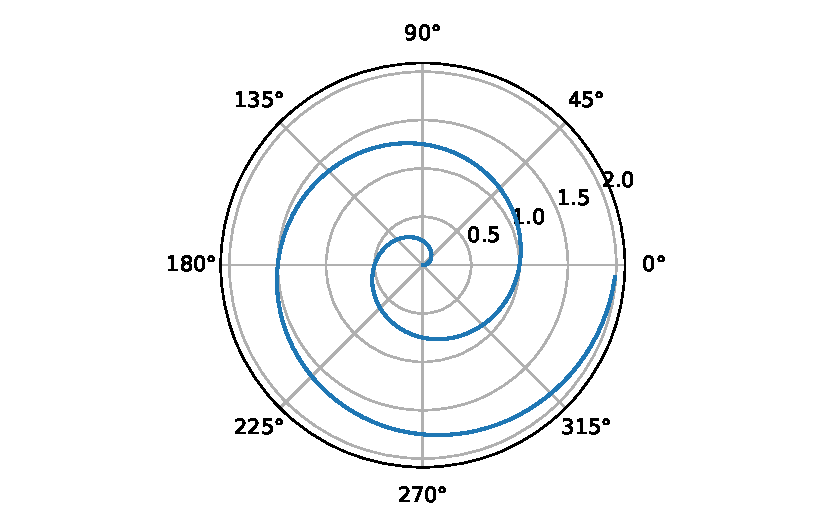
\includegraphics{capitulo_2_files/figure-pdf/fig-chart-1.pdf}

}

\end{figure}%

ver figura~\ref{fig-chart} para \ldots(1)

ver Figura~\ref{fig-chart} \ldots{} (2)

la nominación ``figura x'' es la que predeterminamos en el archivo YAML,
si se quiere colocar en mayúscula el prefijo ``Figura'' como en (2),
solo colocamos {[}Figura @fig-nombredefigura{]} y se obtendrá en
mayúscula, si se quiere hacer lo contrario puede editarlo en el archivo
YAML.

\section{Referenciación de tablas}\label{referenciaciuxf3n-de-tablas}

\begin{longtable}[]{@{}lll@{}}
\caption{Tabla para ver}\label{tbl-letters}\tabularnewline
\toprule\noalign{}
Col1 & Col2 & Col3 \\
\midrule\noalign{}
\endfirsthead
\toprule\noalign{}
Col1 & Col2 & Col3 \\
\midrule\noalign{}
\endhead
\bottomrule\noalign{}
\endlastfoot
A & B & C \\
E & F & G \\
A & G & G \\
\end{longtable}

Vea tabla~\ref{tbl-letters} a hacer muchas cosas

\bookmarksetup{startatroot}

\chapter{Summary}\label{summary}

In summary, this book has no content whatsoever.

\begin{Shaded}
\begin{Highlighting}[]
\DecValTok{1} \SpecialCharTok{+} \DecValTok{1}
\end{Highlighting}
\end{Shaded}

\begin{verbatim}
[1] 2
\end{verbatim}

\bookmarksetup{startatroot}

\chapter*{Referencias}\label{referencias}
\addcontentsline{toc}{chapter}{Referencias}

\markboth{Referencias}{Referencias}

\phantomsection\label{refs}
\begin{CSLReferences}{1}{0}
\bibitem[\citeproctext]{ref-fao}
FAO, F., \& United Nations, A. O. of the. (2010). \emph{Vision general
del sector pesquero nacional del Peru}.
\url{https://www.fao.org/fishery/docs/DOCUMENT/fcp/es/FI_CP_PE.pdf}

\bibitem[\citeproctext]{ref-opesq}
Manrique, A. T. (2010). \emph{DECRETO SUPREMO Nº 016-2003-PRODUCE}.
\url{https://cdn.www.gob.pe/uploads/document/file/3155190/D.S.\%20N\%C2\%BA\%20006-2022-PRODUCE.pdf.pdf}

\end{CSLReferences}



\end{document}
